% COUNT: 510
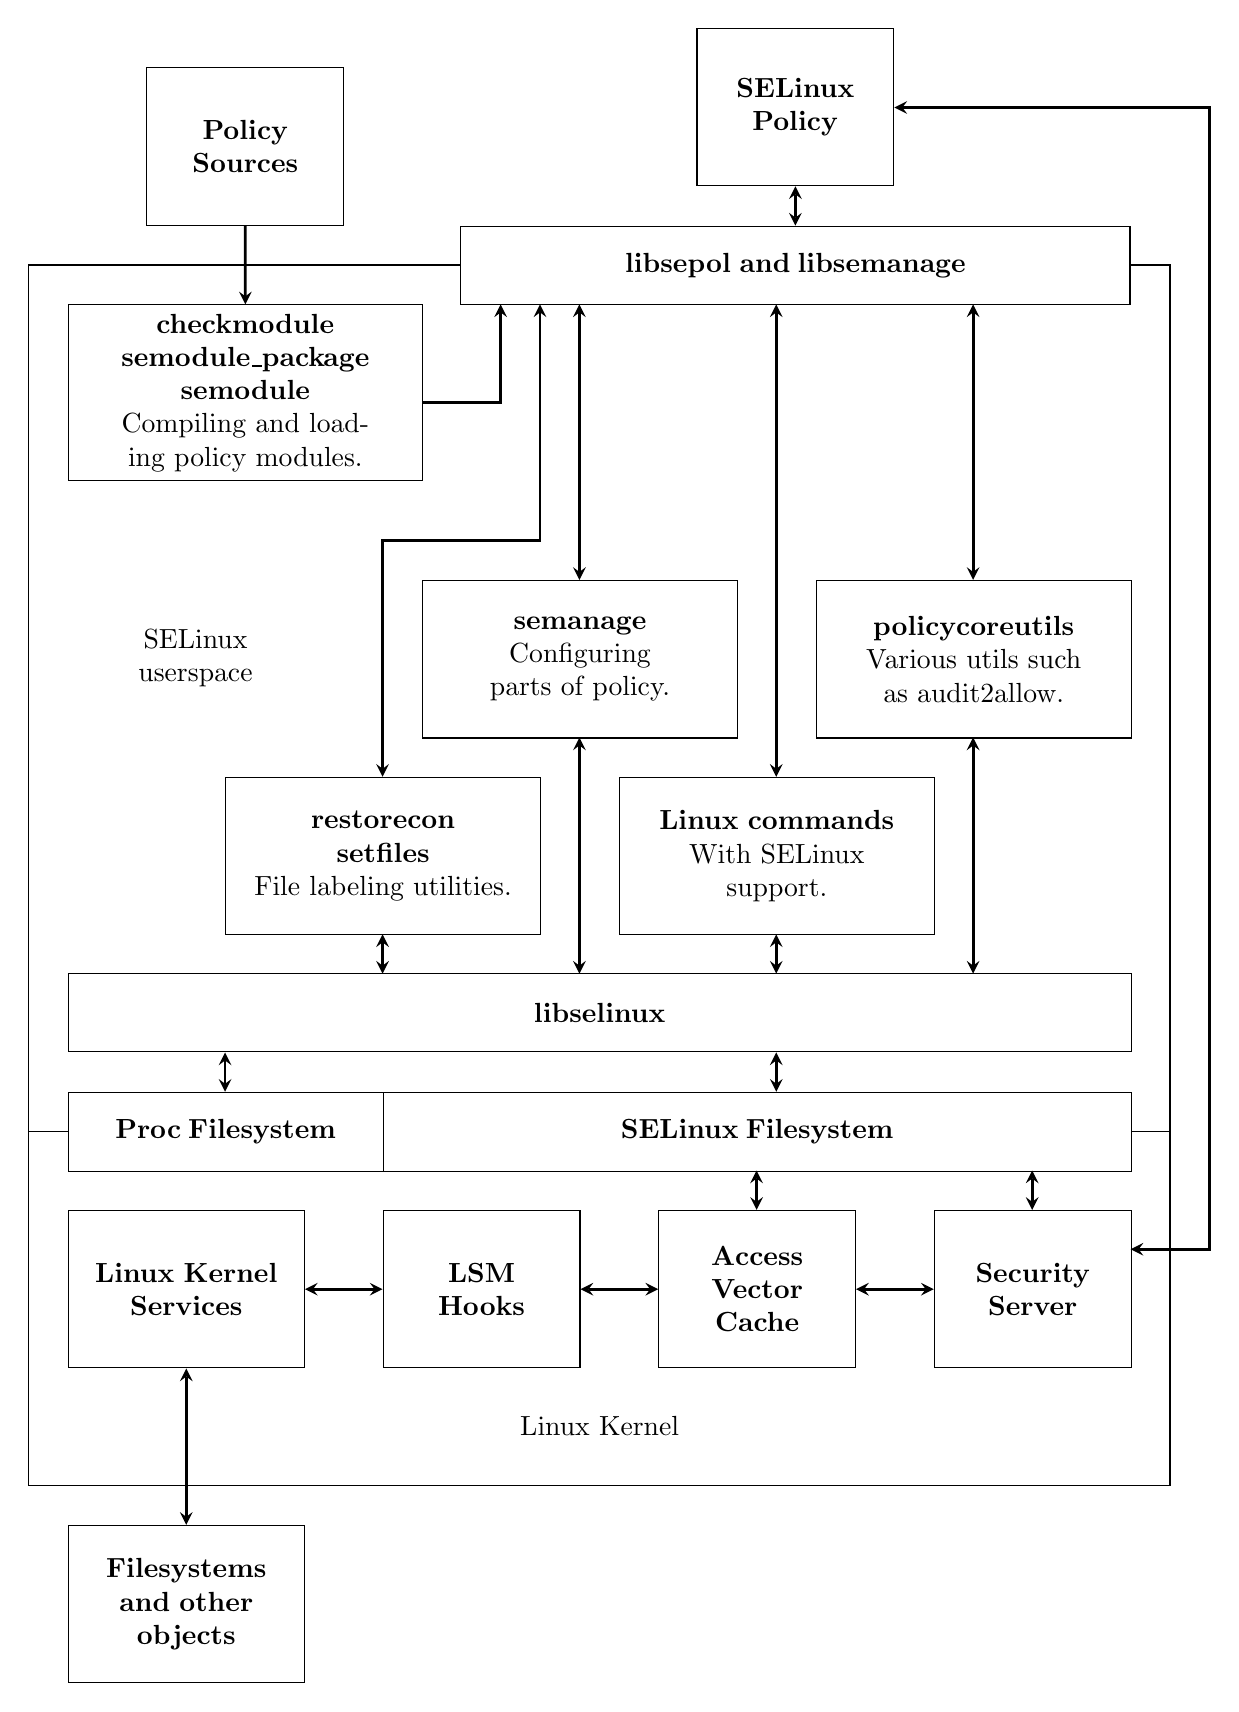
\begin{tikzpicture}
    \usetikzlibrary{calc}
    \tikzstyle{arrow} = [->,>=stealth, line width=1pt]
    \tikzstyle{darrow} = [<->,>=stealth, line width=1pt]
    \tikzstyle{rec} = [rectangle, draw=black, align=center, text width=3.5cm,
        minimum height=2cm, minimum width=4cm, fill=white]

    \draw (0,0) rectangle (14.5,-11);
    \draw (0,-11) rectangle (14.5,-15.5);

    \node(userspace) [rectangle, text width=2cm, align=center]
        at (1,-4.5) [anchor=north west]
        {SELinux userspace};
    \node(kernel) [rectangle, text width=4cm, minimum width=13.5cm,
        align=center]
        at (0.5,-14.5) [anchor=north west]
        {Linux Kernel};

    \node(policysource) [rec, text width=2cm, minimum width=2.5cm]
        at (1.5,0.5) [anchor=south west]
        {\textbf{Policy Sources}};
    \node(compiling) [rec, text width=4cm, minimum width=4.5cm]
        at (0.5,-0.5) [anchor=north west]
        {\textbf{checkmodule\\ semodule\_package\\
        semodule}\\ Compiling and loading policy modules.};
    \node(libsepol) [rec, text width=8cm, minimum width=8.5cm, minimum
        height=1cm]
        at (14,0.5) [anchor=north east]
        {\textbf{libsepol\;and\:libsemanage}};
    \node(policy) [rec, text width=2cm, minimum width=2.5cm]
        at (11,1) [anchor=south east]
        {\textbf{SELinux Policy}};
    \node(semanage) [rec]
        at (5,-4) [anchor=north west]
        {\textbf{semanage}\\ Configuring parts of policy.};
    \node(policycoreutils) [rec, right of=semanage, node distance=5cm]
        {\textbf{policycoreutils}\\ Various utils such as
        audit2allow.};
    \node(restorecon) [rec]
        at (2.5,-6.5) [anchor=north west]
        {\textbf{restorecon\\ setfiles}\\ File labeling
        utilities.};
    \node(linuxcmd) [rec, right of=restorecon, node distance=5cm]
        {\textbf{Linux commands}\\ With SELinux support.};
    \node(libselinux) [rec, text width=13cm, minimum width=13.5cm, minimum
        height=1cm]
        at (0.5,-10) [anchor=south west]
        {\textbf{libselinux}};
    \node(selinuxfs) [rec, text width=9cm, minimum width=9.5cm, minimum
        height=1cm]
        at (4.5,-10.5) [anchor=north west]
        {\textbf{SELinux\:Filesystem}};
    \node(procfs) [rec, text width=3.5cm, minimum width=4cm, minimum
        height=1cm]
        at (0.5,-10.5) [anchor=north west]
        {\textbf{Proc\:Filesystem}};
    \node(kernelservices) [rec, text width=2.5cm, minimum width=3cm]
        at (0.5,-12) [anchor=north west]
        {\textbf{Linux Kernel Services}};
    \node(fs) [rec, text width=2.5cm, minimum width=3cm,
        below of=kernelservices, node distance=4cm]
        {\textbf{Filesystems and other objects}};
    \node(lsmhooks) [rec, text width=2cm, minimum width=2.5cm,
        right of=kernelservices, node distance=3.75cm]
        {\textbf{LSM Hooks}};
    \node(avc) [rec, text width=2cm, minimum width=2.5cm, right of=lsmhooks,
        node distance=3.5cm]
        {\textbf{Access Vector Cache}};
    \node(secser) [rec, text width=2cm, minimum width=2.5cm, right of=avc,
        node distance=3.5cm]
        {\textbf{Security Server}};

    \draw[arrow] (policysource) -- (compiling);
    \draw[darrow] (libsepol) -- (policy);
    \draw[darrow] (fs) -- (kernelservices);
    \draw[darrow] (kernelservices) -- (lsmhooks);
    \draw[darrow] (lsmhooks) -- (avc);
    \draw[darrow] (avc) -- (secser);

    \draw[arrow] (5,-1.75) -- (6,-1.75) -- (6,-0.5);
    \draw[darrow] (6.5,-0.5) -- (6.5,-3.5) -- (4.5,-3.5) -- (4.5,-6.5);
    \draw[darrow] (9.5,-0.5) -- (9.5,-6.5);
    \draw[darrow] (7,-0.5) -- (7,-4);
    \draw[darrow] (12,-0.5) -- (12,-4);
    \draw[darrow] (4.5,-8.5) -- (4.5,-9);
    \draw[darrow] (7,-6) -- (7,-9);
    \draw[darrow] (9.5,-8.5) -- (9.5,-9);
    \draw[darrow] (12,-6) -- (12,-9);

    \draw[darrow] (2.5,-10) -- (2.5,-10.5);
    \draw[darrow] (9.5,-10) -- (9.5,-10.5);
    \draw[darrow] (9.25,-11.5) -- (9.25,-12);
    \draw[darrow] (12.75,-11.5) -- (12.75,-12);
    \draw[darrow] (14,-12.5) -- (15,-12.5) -- (15,2) -- (11,2);
\end{tikzpicture}
